\newcommand{\todo}[1]{\colorbox{yellow}{\textbf{[#1]}}}
\newcommand{\sam}[1]{\textcolor{red}{{\it [Sam says: #1]}}}
\newcommand{\dan}[1]{\textcolor{blue}{{\it [Dan says: #1]}}}


%\documentclass{acm_proc_article-sp}
\documentclass{sig-alternate}

\clubpenalty=10000
\widowpenalty = 10000

%\documentclass{sig-alternate-2014}
\newfont{\mycrnotice}{ptmr8t at 7pt}
\newfont{\myconfname}{ptmri8t at 7pt}
\let\crnotice\mycrnotice%
\let\confname\myconfname%


\permission{Permission to make digital or hard copies of all or part of this work for personal or classroom use is granted without fee provided that copies are not made or distributed for profit or commercial advantage and that copies bear this notice and the full citation on the first page. Copyrights for components of this work owned by others than ACM must be honored. Abstracting with credit is permitted. To copy otherwise, or republish, to post on servers or to redistribute to lists, requires prior specific permission and/or a fee. Request permissions from permissions@acm.org.}
\conferenceinfo{SIGCSE'14,}{March 3--8, 2014, Atlanta, GA, USA.}
\copyrightetc{Copyright 2014 ACM \the\acmcopyr}
\crdata{978-1-4503-2605-6/14/03\ ...\$15.00.\\
%http://--enter the whole DOI string from rightsreview form confirmation
}



\usepackage{cite}
%\usepackage{hyperref}
\usepackage{listings}
\usepackage{booktabs}
\usepackage{color}
\usepackage{array}
\usepackage{subfigure}
\usepackage{balance} % Add this back in. Probably needed during camera ready.
\usepackage{tikz}
\usepackage{pgfplots}

%%%% Needed packages?
%\usepackage{graphicx}
%\usepackage{times}  % Is this needed?
%\usepackage{xspace}
%\usepackage{multirow}
%\usepackage{tabularx}
%\usepackage{subfigure}
%\usepackage{fancybox}

\pgfplotsset{compat=1.4}

\usepackage{listings}

%\usepackage[papersize={8.5in,11in}]{geometry}

\pdfpagewidth=8.5in
\pdfpageheight=11in

\begin{document}

% Is this needed?
%\conferenceinfo{SIGCSE}{'2014 Atlanta, Georgia, USA}

\title{Using a Real World Project in a Software Testing Course}

\numberofauthors{1} %  in this sample file, there are a *total*
% of EIGHT authors. SIX appear on the 'first-page' (for formatting
% reasons) and the remaining two appear in the \additionalauthors section.
%
\author{
%
% 1st. author
\alignauthor
Daniel E. Krutz, Samuel A. Malachowsky, and Thomas Reichlmayr\\ 	
	\affaddr{Software Engineering Department}\\
       \affaddr{Rochester Institute of Technology}\\
       \affaddr{1 Lomb Memorial Drive}\\
       \affaddr{Rochester, NY 14623} \\
       \email{\{dxkvse, samvse, tjrese\}@rit.edu}
% 2nd. author
%\alignauthor
%Danie2 E. Krutz\\ 	
%	\affaddr{Software Engineering Department}\\
    %   \affaddr{Rochester Institute of Technology}\\
     %  \affaddr{1 Lomb Memorial Drive}\\
     %  \affaddr{Rochester, NY 14623} \\
     %  \email{dxkvse@rit.edu}
% 3rd author
%\alignauthor
%Danie2 E. Krutz\\ 	
%	\affaddr{Software Engineering Department}\\
  %     \affaddr{Rochester Institute of Technology}\\
   %    \affaddr{1 Lomb Memorial Drive}\\
    %   \affaddr{Rochester, NY 14623} \\
     %  \email{dxkvse@rit.edu}
} % Must not be a space above this


\maketitle
\begin{abstract}

Although testing often accounts for 50\% of the budget of a typical software project, the subject of software testing is often overlooked in computing curriculum. Students often view testing as a boring and unnecessary task, and education is usually focused on building software, not ensuring its quality. Previous works have focused on either making the subject of testing more exciting for students or on a more potent lecture-based learning process.

At the Department of Software Engineering at the Rochester Institute of Technology, recent efforts have been focused on the project component of our Software Testing course as an area of innovation. Rather than previous methods such as a tightly controlled and repetitive testbed, our students are allowed to choose a real-world, open source project to test throughout the term. With the instructor as both counsel and client, students are expected to deliver a test plan, a final report, and several class-wide presentations.

This project has achieved significant student praise; qualitative and quantitative feedback demonstrates both increased satisfaction and fulfilled curricular requirements. Students enjoy the real-world aspect of the project and the ability to work with relevant applications and technologies. This paper outlines the project details and educational goals.


\end{abstract}

%\todo{define the categories and fix the keywords \& terms}
% A category with the (minimum) three required fields
%\category{H.4}{Information Systems Applications}{Miscellaneous}
%A category including the fourth, optional field follows...
%\category{D.2.8}{Software Engineering}{Metrics}[complexity measures, performance measures]


\category{K.3.2}{Computers and Education}Computers and Information
Science Education- Computer science education; Curriculum

\terms{Design, Reliability, Verification}

% My best show at keywords
\keywords{Software Testing, Software Engineering Education, Software Project}

\section{Introduction}

Software testing is an important aspect of creating reliable software. Defects can have numerous adverse affects on an application, ranging from unhappy customers and users to injury or even death. Projects should place a more significant focus on testing; recent studies have indicated that testing makes up over 50\% of the cost of a typical software project~\cite{Osterweil:1996:SDS:242223.242288} and a third of the cost of all software bugs could be eliminated through improved testing~\cite{5876141}. Unfortunately, testing is far too often overlooked in both industry and academia.

Software Engineering education is far too often deficient in this area as well. Although most universities have programs in computing, very few offer courses with a primary focus in software testing~\cite{krutz_BotD}~\cite{Myers:2004:AST:983238}~\cite{Shepard:2001:MTT:376134.376180}. Additionally, the educational mindset of most schools is to teach students how to build software, not break it~\cite{Meneely:2013:VDC:2486788.2486948}.
Largely due to the difficulty of grading such a component or a lack of course time, testing often comprises only a minor portion of the student's grade in the majority of programming courses~\cite{Smith:2012:UPR:2361276.2361295}~\cite{Kazemian:2005:STC:1113847.1113876}. Students often lack enthusiasm about testing; they are usually much more interested in building software than in ensuring its quality~\cite{Clark:2004:PTS:979968.979974}. Finally, testing as both a concept and a practice can be very difficult to teach through lectures. Kaner~\emph{et al.}~\cite{4271602}  stated that ``the challenge is to develop group activities that can foster insight---a level of abstract understanding that can apply from situation to situation---rather than emphasizing detailed procedural understanding.''

There is a significant amount of research which shows the importance of software testing, with a substantial amount of improvement needing to be done in both academia and industry~\cite{Osterweil:1996:SDS:242223.242288}~\cite{4722985}. Additionally, software testing in our educational institutions needs to have a more practical focus with educators doing a better job readying their students for industry~\cite{Whittaker:2000:STW:624635.626090}~\cite{Jones:2001:PTS:374824.374715}.

At the Rochester Institute of Technology (RIT), we have offered an upper division Software Testing course since 1998, with a wide focus including process, tools, and analysis. A project component has always been a significant portion of this course, but it became obvious that improvements needed to be made. We have recently altered this project to more directly address a lack of student enthusiasm regarding testing, the desire for students to work on a real-world project, and the need for students to become better acclimated with contemporary testing technologies.

In this paper, we describe an innovative approach to teaching software testing through a project component. Under the supervision of the instructor, who also plays the role as customer, small student teams first choose a moderately sized open source project. Each team then develops a test plan to be followed for the rest of the project term and proceeds to test the chosen application using this plan. Teams give presentations throughout the term to report their progress. The project culminates with a final presentation and test report.

This updated project component has been included in several class offerings and has had substantial success. Students have stated that it has not only significantly increased their knowledge of software testing as a discipline, but of its value as well. Feedback has shown praise both for the real-world nature of the project and the reinforcement it gave to the need for testing.

The remainder of this paper is organized as follows. Section~\ref{sec: aboutcourse} describes the Software Testing course with its general structure and main components. Section~\ref{sec: aboutproject} provides an overview of the project. Section~\ref{sec: sampleproject} discusses a sample student project. Section~\ref{sec: projectresults} discusses project results. Section~\ref{sec: studentfeedback} offers student feedback based on the project. Section~\ref{sec: relatedwork} describes related work. Section~\ref{sec: futurework} discusses future work on the project, and section~\ref{sec: summary} provides a summary of this work.

\section{About the course}
\label{sec: aboutcourse}

Primarily comprised of upper division Software Engineering students, the Software Testing course is also offered to other programs including Computer Science, Computer Engineering, Electrical Engineering, and Game Design. The only prerequisite for our testing course is an earlier class which introduces basic concepts of software engineering including teamwork, development processes, and proper documentation. In this prerequisite Introduction to Software Engineering course, students have already been introduced to some aspects of testing, including unit testing, system testing, integration testing, and acceptance testing. In many cases, other non-required courses and a required one-year cooperative internship (co-op) have exposed students to various aspects of testing as well. The Software Engineering department considers the 3-credit Software Testing course to be the primary means of fully exploring software testing and closely related disciplines.

The course has three primary learning outcomes: to instruct students on the importance of software testing, to expose them to various testing-related tools and techniques, and to explain and exercise the decision process and situations in which certain tests should and should not be used. While various tools such as jUnit\footnote{http://junit.org/}, DJUnit\footnote{http://works.dgic.co.jp/djunit/}, jMock\footnote{http://jmock.org/}, and Selenium\footnote{http://docs.seleniumhq.org/} are discussed throughout the course, it is their underlying categorization and appropriate use that is emphasized. The studies regarding the importance of testing are expounded both by looking at use cases that illustrate a need for testing  and by exploring why testing is often neglected by development teams.

While most students do not become overly enthralled with software testing, we do expend effort to dispel the myth that testing is the bland, monotonous field that many believe it to be. While approximately half of each classroom session is devoted to a lecture, the remaining time is reserved for a relevant hands-on activity or discussion. As an example, each class begins with an interactive "Bug of the Day" (BotD) activity~\cite{krutz_BotD} in which students study a real world software bug, its impacts, and the ways it could have been avoided.  This activity is designed to highlight common bugs and practical application of course topics to actual examples.

Students are graded on several criteria. Each term there are three exams, several homework assignments, and a project based component. Class size is typically 25-40 students.


\section{About the project}
\label{sec: aboutproject}

The Software Testing course at RIT has always had a significant project component. Previously, the project involved all student groups being assigned the same set of code in which they were expected to find known bugs. The tools and testing techniques they were allowed to use was restricted, and the project was largely viewed as bland and unexciting for the students. They did not enjoy working on the same cookie cutter project, wanted something more realistic, were interested in making a real-world contribution, and wanted something that would look better to potential employers. In order to address these concerns and to meet educational goals, we decided to create a new project for the course.

During the first week of the 15 week term, teams are formed. Students are able to assist in the team creation process by choosing which other students they would like to be partnered with. Team size is targeted to 4-6 students, as this is often the size of groups in industry and has been found to be conducive to student learning in previous research~\cite{Guo:2009:GPS:1516546.1516579}~\cite{Petkovic:2006:TPS:1140123.1140202}.

Once the teams have been formed, their first step is to choose an application to be tested. Students are asked to select medium-sized open source applications for testing. They must be large enough to provide an adequately sized test bed, but not so large as to overwhelm the teams. Applications with roughly 100-200 classes have been found to be appropriate for this project, and students are not limited by programming language, even if the instructor is not familiar with the chosen language. Projects with a high level of documentation are preferred, as this provides a basis for acceptance tests and the documentation itself can also be tested. The final step in the application selection process is to have the program approved by the instructor. This must be done by week 3.

The next major deliverable, due in week 5, is the project test plan. Students are provided with an initial template, but test plans are expected to significantly differ from one another due to the wide variety of applications selected. Groups are encouraged to make the best test plans possible, but are not necessarily held to them during the remainder of the course term. Because of expected but unforeseen hurdles as well as new concepts covered in class, students are allowed to build on to and deviate from this test plan as necessary.

\begin{table}[h!]
\caption{Discovered Defect Types}
\begin{center}
    \begin{tabular}{ l | l }
    \toprule

	\bfseries Week & \bfseries Deliverable  \\ \hline \hline
	\bfseries 1 & Teams Formed \\ \hline
	\bfseries 3 & Application Chosen \\ \hline
	\bfseries 5 & Test Plan  \\ \hline
	\bfseries 5-15 & Plan Execution \\ \hline	
	\bfseries 6 & Plan Presentations  \\ \hline
	\bfseries 10 & Progress Report \\ \hline
	\bfseries 15 & Final Report \& Presentation \\ \hline
	\bfseries 15 & Postmortem \\ \hline
% \bottomrule

    \end{tabular}
\end{center}

\label{table:discovereddefecttypes}
%\vspace{-0.3in}
\end{table}

In week 6, each team presents their test plan, along with any results already gathered by the team. This gives the teams an opportunity to receive feedback from their peers, gain valuable public speaking experience, and exposure for their classmates to new testing tools and techniques (which they may use on their own projects). After the presentation, a question and answer session takes place in which students must often defend the choices made for their project. Additionally, students must write a 2-4 page reflection document describing what has and has not gone well so far. A primary objective of this reflection is to allow the students to understand and continue to build upon their strengths while also identifying and remedying areas of improvement. Groups are expected to perform a critical analysis of these findings and propose resolutions for problematic areas.

In week 10 of the term, groups are asked to submit a brief report detailing their progress to that point. This deliverable serves two purposes: it gives the instructor insight with an opportunity to intervene, and it provides a milestone for groups mid-project.

In the final week, students submit their final report, which details not only the findings of their testing, but also the specific tests used and relevant data. Students are also encouraged to state why they chose and carried out particular tests and provide a rationale for the processes and techniques they employed. They are not expected to propose resolutions for the discovered bugs, as this could violate the intent of the exercise and serve to distract the team. Groups are, however, encouraged to identify the steps needed to duplicate the defect, which appropriately represents the similar action needed in industry to resolve defects. Much like in week 6, students again present their findings to the rest of the class, including a 5-10 minute window for questions and answers.

The final project deliverable is a postmortem. In this document, students reflect on what went well, what went poorly, and how they could improve upon each. This critical analysis is also expected to contain possible resolutions for all difficulties encountered along the way.

Grading of all deliverables is done using a rubric. The presentations, for example, are evaluated on how well they prepared, the quality of project information conveyed to the class, and how well they answered project questions. No significant part of the grading is based upon the number of bugs found by a team, as students are encouraged to be more concerned with the processes and techniques they are using rather than the number of defects they discover.


\section{Sample project}
\label{sec: sampleproject}

% Maybe discuss a second student project if we need room to bulk up the paper

As stated in the last section, the primary criteria for selection were size and a restriction to open-source projects. Students selected a wide range of open source applications, including both traditional and mobile applications, applications written for Unix, Windows, and OSX operating systems, and applications written by both small groups and organizations the size of Mozilla. A few of the tested applications included JBrick~\footnote{http://code.google.com/p/jbrick/}, tuxGuitar~\footnote{http://sourceforge.net/projects/tuxguitar/},  Notepad++~\footnote{http://notepad-plus-plus.org} and components of Firefox~\footnote{http://www.mozilla.org/en-US/firefox/}.

In the following example, we will discuss an example student testing project which analyzed jBrick, an application designed to assist handicapped students in programming Lego robots. The group was comprised of 6 students, 3 of which had previously indicated that they wished to work together. Because one of the team members had previous experience with jBrick, it was chosen as the test application after a brief team discussion.

The students were able to gather both the source code and a significant amount of documentation from the jBrick project website. Their initial plan was largely devoted to usability and acceptance testing of the project. While these tests would have yield some results, instructor feedback indicated that they should explore a wider variety of applicable tests, keeping in mind the cost/benefit trade-off in their choices.

The team ultimately decided to add unit and mutation testing. They met twice a week for 1-2 hours and stayed in touch via text, Google Docs, and social media. The team regularly met with the instructor who played both the role of teacher and customer for the project. During their final presentation, they indicated that they had performed most of their intended testing on the application, but were unable to perform some of the unit tests due to time constraints and some of the mutation testing due to technical limitations.

The team's testing revealed some compelling results. Since jBrick was intended for both the visually and non-visually impaired, usability testing was performed on the application using representatives of both groups. While some usability issues were identified by visually impaired users, a surprisingly higher number were found by non-impaired users. Additional issues found included negative application performance due to poorly written code and functions which needed repair (revealed in unit testing).

In their postmortem, the team indicated that although they believed their project went well, they felt there was room for significant improvement in both their testing methodologies and their team dynamics. The team expressed that they should have used more automated testing tools to reduce the monotony of some of the tests as well as a wider variety of tests, including fuzz testing. The team also stated that they should have met more as a group and stayed in closer contact with one another throughout the course of the project. Members indicated that lack of communication significantly hindered their team's performance.


\section{Project Results}
\label{sec: projectresults}

Students have uncovered a wide variety of bugs with varying levels of severity. Table~\ref{table:discovereddefecttypes} shows some of the types of bugs discovered by 18 groups spanning several course offerings with each group testing a unique project. Instructors should remember that all projects are different and that the types and number of defects students discover will significantly vary. All examined projects are different and a properly developed testing process does not necessarily lead to the discovery of a large number or variety of defects.


\begin{table}[h!]
\caption{Discovered Defect Types}
\begin{center}
    \begin{tabular}{ l | l }
    \toprule

	\bfseries Type of bug & \bfseries \# Found  \\ \hline \hline
	\bfseries Minor, non-functional & 153 \\ \hline
	\bfseries Incorrect Documentation & 287 \\ \hline
	\bfseries Poor Usability & 113  \\ \hline
	\bfseries Incorrect Functionality & 49  \\ \hline
	\bfseries Crash & 35 \\ \hline
% \bottomrule

    \end{tabular}
\end{center}

\label{table:discovereddefecttypes}
%\vspace{-0.3in}
\end{table}

The majority of issues discovered have been relatively minor, such as grammar mistakes, inadequate documentation, and poor usability. In most cases, however, students were able to find significant numbers of more serious issues such as crashes in the application and functionality that was incorrect. In measuring the severity of defects, teams studied the accuracy of results and if requirements were met or failed.

Students were able to find bugs using a wide variety of testing tools and technologies. Table~\ref{table:typesoftesting} includes a list of those most frequently chosen by the students. The majority of teams chose to conduct unit, acceptance, usability, and compatibility testing. While these tests were certainly good choices, it is likely that teams selected them because they were both relatively easy to implement and students had been exposed to them early in the course.

\begin{table}[h!]
\caption{Types of Testing Conducted by Teams}
\begin{center}
    \begin{tabular}{ l | l }
    \toprule

	\bfseries Type of test & \bfseries \# Found  \\ \hline \hline
	\bfseries Unit & 16 \\ \hline
	\bfseries Acceptance & 17 \\ \hline
	\bfseries Usability & 17 \\ \hline
	\bfseries Fuzz & 10 \\ \hline
	\bfseries Accessibility & 8 \\ \hline
	\bfseries Security & 3 \\ \hline
	\bfseries Performance & 10 \\ \hline
	\bfseries Compatibility & 18 \\ \hline
%	\bfseries a & x \\ \hline

    \end{tabular}
\end{center}

\label{table:typesoftesting}
%\vspace{-0.3in}
\end{table}

After completion, most teams chose to submit their bug reports to the application's development team. Several have received messages from the developers thanking them and confirming the existence of the errors they had discovered.

% Several open source projects have been notified of bugs and have acknowledged their existence
% Students have indicated that it demonstrates the importance of proper documentation. This is something that is a difficult concept to drive home to students.


\section{Student Feedback}
\label{sec: studentfeedback}

Students have expressed a significant amount of satisfaction in this project and it has contributed to their overall satisfaction with the course. At the conclusion of the term, students are asked to submit an anonymous survey rating several aspects of the course, instructor, and project. Several of these questions and student responses are shown in Table~\ref{table:studentfeedback}. These questions have been posed to students in the last three course offerings, all of which have used this project component. A total of 78 students from these sections have responded to the survey.

\begin{table}[h!]
\caption{Student Responses}
\begin{center}
    \begin{tabular}{ l | l | l | l    }
    \toprule

	\bfseries & Yes & \bfseries No & \bfseries Total \\ \hline \hline
	\bfseries Did you enjoy the software project? & 66 & 12 & 85\%  \\ \hline
	\bfseries Would you recommend this project? & 60 & 18 & 77\%  \\ \hline
	\bfseries Resembles a real world project? & 60 & 18 & 77\%  \\ \hline
	\bfseries How much did you learn? (0-5)& - & - & 4.15  \\
 \bottomrule
    \end{tabular}
\end{center}

\label{table:studentfeedback}
%\vspace{-0.3in}
\end{table}

These results indicate that the vast majority of students not only enjoyed the project, but would also recommend it to a classmate as well. Additionally, most students felt that it reassembled a project which they were likely to encounter in the real world and were similar to tasks they were asked to complete while on co-op. Finally, students were asked to rate how much they learned from the project on a 0-5 scale, with 0 representing them learning very little and 5 representing the maximum amount of learning. The average student response was a 4.15/5 indicating that, on average, students felt the project to be very educational.

The end of term feedback also allowed students to write some of their thoughts regarding the course project. The following are samples of written feedback that have been received:

\begin{quotation}
``The Software Testing course helped to drive home the importance of testing at every stage in the software development life cycle. The project component was especially helpful in this area. We were able to see the abundance of errors that existed even in our favorite applications.''
\end{quotation}

\begin{quotation}
``Testing one of my favorite open source applications helped to keep me interested in the project. Not only was I able to examine the source code of a tool I regularly used, but it made me feel good to know that I was assisting in removing defects from a tool I used on a regular basis, for both myself and other open source users as well. ''
\end{quotation}

\begin{quotation}
``Testing is a difficult, time consuming and sometimes monotonous process. It is however, very important. I was shocked by all the bugs our team discovered in what I thought to be a heavily tested and defect free application.''
\end{quotation}

\begin{quotation}
``Like with many aspects of software engineering, software testing is heavily process based. Before this project, I viewed testing as an ad-hoc process that waited until the conclusion of a project. This project has taught me the importance of documentation and process in software testing. Additionally, I've learned that testing should occur at numerous stages in software development.''
\end{quotation}

After taking the course and returning from co-op, students have stated they this course project prepared them very well for projects which they worked on in industry. The project has also helped to increase specific interest in software testing for several students, some of which have subsequently taken full time jobs in the field of software testing. Many students have reported that they were able to gain a co-op or full time job in a field of software testing or a related discipline largely from their experiences with this project.

The enthusiasm students have about the project has also been stated as a major reason why many decide to enroll in the class. One testament to this is the growing enrollment figures for the elective course. The first term in which the new project was offered was in the Fall of 2010. Since this offering, student enrollment figures have progressively increased for the course. The second offering of 2012 saw the maximum number of students allowed for a course, 40, to be reached, leaving numerous students on the waiting list unable to attend. While it is impossible to unequivocally state that the project is the sole reason for the increased student enrollment figures, we believe that these numbers act as yet another testament for student enthusiasm regarding the project. It is possible that the enthusiasm of the class instructors regarding the new project and its inherent variative nature has been a factor in student satisfaction as well. A chart representing student enrollment for the course since 2008 is shown in Figure~\ref{fig:enrollmentchange}. The line in the chart represents when the project was first offered as part of the course.

% Figure 1 is hardcoded
\begin{figure}[h!]
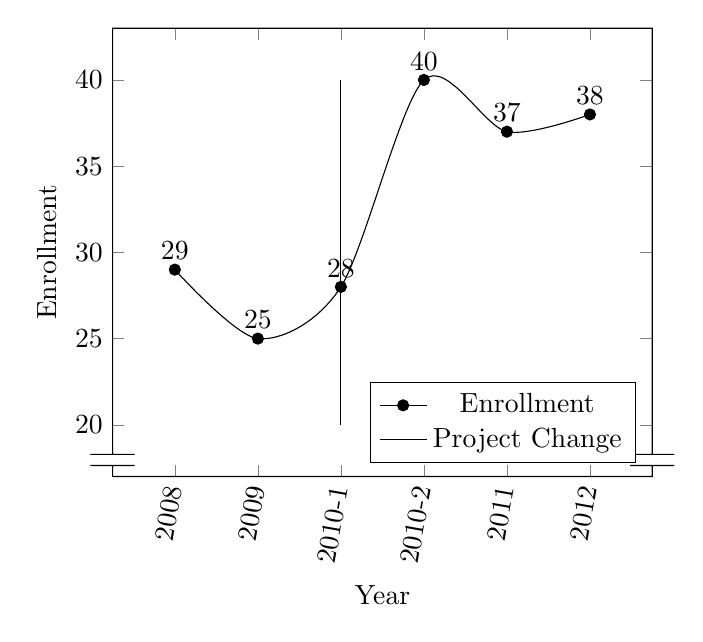
\begin{tikzpicture}
\begin{axis}[
   smooth,
   enlargelimits=0.15,
	xlabel={Year},
   ylabel={Enrollment},
  symbolic x coords={2008, 2009, 2010-1, 2010-2, 2011, 2012, 2013},
 xtick=data,
  x tick label style={rotate=80,anchor=east},
  legend pos=south east,
 axis y discontinuity=parallel,
  ]	
\addplot+[nodes near coords, draw=black, mark options={solid,color=black}] plot coordinates {(2008,29) (2009,25) (2010-1,28) (2010-2,40) (2011,37) (2012,38)};
\addlegendentry{Enrollment}

\addplot+[mark=none, draw=black] coordinates {(2010-1,20) (2010-1,40)};
\addlegendentry{Project Change}
\label{axis:studentenrollment}
\end{axis}
\end{tikzpicture}

\caption{Student Enrollment Change}
\label{fig:enrollmentchange}
\end{figure}


\section{Related Work}
\label{sec: relatedwork}

There have been numerous works which have stated the need of further emphasis on software testing education~\cite{Clark:2004:PTS:979968.979974}~\cite{4271602}~\cite{Edwards:2003:TST:949344.949431}.  Some the deficiencies in software testing education include the inability to excite students about the topic, lack of relevant projects for students to interact with, and a primary educational focus on building rather than breaking software~\cite{Meneely:2013:VDC:2486788.2486948}~\cite{Harrison:2010:TST:1858583.1858591}~\cite{Clark:2004:PTS:979968.979974}.

In order to assist software testing education, previous works have focused on enhancing the education process either through making it more exciting for students, or through a more educational experience. Gotel~\emph{et al.}~\cite{Gotel:2008:TSQ:1597849.1384329} described the use of an open source web-based system for teaching software testing. This project revolved around having student-created problems which other students were expected to solve. Elbaum~\emph{et al.}~\cite{Elbaum:2007:BHM:1248820.1248899} created a web-based tutorial known as Bug Hunt. The goal of this hands on activity was to teach students software testing at their own pace. Tutorials provided instant feedback to the user and automatically assessed the student's performance.

Preston~\cite{Preston:2005:UAR:1869667.1869671} described the use of real-world projects in Information Technology education. The use of such projects was found to allow students to apply the theoretical knowledge they previously learned and solidify their understanding of the subject matter. Harrison~\cite{Harrison:2010:TST:1858583.1858591} described a method of teaching software testing using viewpoints from both the developer and the software tester. This approach is beneficial since this allows students to see the importance and impact of proper software testing from each perspective. Goldwasser~\cite{Goldwasser:2002:GIS:563517.563446} described several fun and innovative methods of including software testing into a curriculum. In one example, students acted in a competitive fashion against a common test set.

\section{Future work}
\label{sec: futurework}



This project has been utilized in several sections of our Software Testing course and has been very successful, but there are enhancements which may be done to the project and further data which may be collected. One of the main purposes of the project is to allow a significant amount of freedom for each project team while achieving stated educational goals. While project deliverables are defined, each team is allowed to assign their own team roles, select their own projects, and choose the tests to run on the target application. The opportunity to make their own decisions and learn how to self-manage team in a supervised setting has presented some issues. Some of the teams have struggled with the extent of afforded freedom and have requested an extra deliverable and guidance during the term. In future implementations of this project, an extra deliverable will be added in week 10 which will include a written status and brief presentation. Finally, in past iterations some teams have been comprised of as many as 6 students; in the future, groups will be limited to 4-5 students to make meeting scheduling and communication demands more manageable.

This type of real world project is applicable to other educational areas of computing and may be applied to these courses as well. As an example, a software security course could implement a similar project to check for vulnerabilities in open source applications and propose fixes. A software design course could review the design of an application including the positive or negative ramifications of that design. In order to further measure the effectiveness of the project outlined above, we would like to poll seniors who took the Software Testing course regarding the effect of the project had on their subsequent experiences with software testing (i.e. co-op and senior capstone).

\section{Summary}
\label{sec: summary}
Software Engineers need to understand the importance of developing high quality, defect free software. In order to ensure students are prepared for this task, we have developed an innovative software testing project which closely resembles tasks students will face upon graduation.

We have witnessed a significant increase in student enthusiasm in software testing as a subject and a discipline. This is largely due to us allowing students to select contemporary real world projects to test. Students have generally found the project to be very educational and feedback has indicated that it been a significant asset to them in industry. At least two other universities are planning to incorporate a similar project in their Software Testing classes and we encourage others to consider this approach in their courses as well.


%\end{document}  % This is where a 'short' article might terminate
\balance
\bibliographystyle{abbrv}
\bibliography{testingprojectrefs}  % sigproc.bib is the name of the Bibliography in this case

%\balancecolumns
% That's all folks!
\end{document}



% Todo
%- Software Testing or software testing course ? - Capatlize when referring to the class
%-
% \todo{educational goals change to learning outcomes or course objectives}

% % ``Not a Clone'' 